\documentclass{beamer}
\usetheme{CambridgeUS}

%\documentclass[handout]{beamer}
%\usetheme{Pittsburgh}
%\beamertemplatesolidbackgroundcolor{black!2}
%\setbeamertemplate{footline}[frame number]
%\usepackage{pgfpages}
%%\pgfpagesuselayout{4 on 1}[a4paper,border shrink=5mm,landscape]
%\pgfpagesuselayout{8 on 1}[a4paper,border shrink=5mm]

%%% PACKAGES
\usepackage[russian]{babel}
\usepackage[utf8]{inputenc}
\usepackage{amsmath}
\usepackage{amssymb}
\usepackage{tikz}
\usepackage{graphics}
\usepackage{appendixnumberbeamer}

%%% BEAMER SETTINGS
\setbeamertemplate{navigation symbols}{}
\setbeamertemplate{headline}{}

%%% TIKZ SETTINGS
\usetikzlibrary{fit}

%%% NEW COMMANDS
\def\pitem{\pause \item}

\DeclareGraphicsRule{.1}{mps}{*}{}
\DeclareGraphicsRule{.2}{mps}{*}{}
\DeclareGraphicsRule{.3}{mps}{*}{}
\DeclareGraphicsRule{.4}{mps}{*}{}
\DeclareGraphicsRule{.5}{mps}{*}{}
\DeclareGraphicsRule{.6}{mps}{*}{}

%\includeonlyframes{current} % leaves only the given frames

\title[Недоминирующая сортировка]{Разработка гибридного алгоритма недоминирующей сортировки}
%\transduration{20}
\author[Маргарита Маркина]{Маргарита Маркина}
\institute[]{Национальный исследовательский университет информационных технологий, механики и оптики}
\date{}

\begin{document}

\begin{frame}
%\transduration{20}
\begin{center}
{\scriptsize Санкт-Петербургский национальный исследовательский университет \\ информационных технологий, механики и оптики}

\vspace{1cm}

{\scriptsize Факультет информационных технологий и программирования

Кафедра компьютерных технологий}

\vspace{1cm}

\vbox{\large\bfseries
Разработка гибридного алгоритма недоминирующей сортировки}

\vspace{1cm}

{\large Маркина Маргарита Анатольевна \\}
{\large Группа M3438}


\vspace{1cm}

{\large Научный руководитель: к.т.н. доцент кафедры КТ \\}
{\large М.~B.~Буздалов}


\end{center}
\end{frame}

%%%%%%%%%%%%%%%%%%%%%%%%%%%%%%%%%%%%%%%%%%%%%%%%%%%%%%%%%%%%%%%%%%%%%%%%%%%%%%%%%%%%%%%%%%%%%%%%%%%%%%%%%%%%%%%%%%%%%%%%
%\frame[label=title]{\titlepage}

\begin{frame}{Решаемая проблема}
%\transduration{20}
\begin{block}{Предметная область}
\begin{itemize}
\item Недоминирующая сортировка.
\item Многокритериальная задача оптимизации.
\item Гибридизация алгоритмов.
\item Оценка времени работы алгоритмов.
\end{itemize}
\end{block}
\end{frame}

\begin{frame}{Решаемая проблема}
%\transduration{20}
\begin{block}{Введение}
\begin{itemize}
\item Точка $A=(a_1,...,a_M)$ доминирует точку $B=(b_1,...,b_M)$, \\
когда $\forall ~ 1 \leq i \leq M : a_i \leq b_i$ и $\exists j : a_j < b_j $.
\item \textit{Недоминирующая сортировка} множества точек $S$ в $M$-мерном пространстве — это процедура, назначающая всем точкам из $S$ \textit{ранг}.
\item Все точки, которые не доминируются ни одной точкой из $S$, имеют ранг 0.
\item Точка имеет ранг $i+1$, если максимальный ранг среди доминирующих  её точек равен $i$.
\end{itemize}
\end{block}
\end{frame}


\begin{frame}{Решаемая проблема}
%\transduration{20}
\begin{block}{Введение}
На рисунке 3 фронта: 

$\{a, b, c, d\}$ имеет ранг 0, $\{e, f\}$ - ранг 1, $\{g, h, i\}$ - ранг 2.
\begin{center}
\includegraphics*[height=6cm]{pic/non_dominated_sort.png}
\end{center}
\end{block}
\end{frame}

\begin{frame}{Решаемая проблема}
%\transduration{20}
\begin{block}{Актуальность}
\begin{itemize}
\item Многокритериальные эволюционные алгоритмы. 
\item Задача минимазациии.
\end{itemize}
\end{block}
\end{frame}


\begin{frame}{Решаемая проблема}
%\transduration{20}
\begin{block}{Цель исследования}
\begin{itemize}
\item Выбрать наиболее подходящие алгоритмы.
\item Выявить преимущества каждого алгоритма.
\item Научиться по входным данным выбирать стратегию.
\item Сделать гибридный алгоритм.
\end{itemize}
\end{block}
\end{frame}


\begin{frame}{Решение}
%\transduration{20}
\begin{block}{Fast + BOS}
\begin{center}
%\includegraphics*[height=3cm]{pic/illustrations.6}
\end{center}
\begin{itemize}
\item Fast Version of the Generalized Algorithm. 
%\item Сделать нормальное назввние TODO 
\item Best Order Sort.
\end{itemize}
\end{block}
\end{frame}

\begin{frame}{Решение}
%\transduration{20}
\begin{block}{Fast}
\begin{center}
%\includegraphics*[height=3cm]{pic/illustrations.6}
\end{center}
\begin{itemize}
\item Fast Version of the Generalized Algorithm.
\begin{itemize}
\item Разделяй и властвуй по $N$ и $M$. 
\item На каждом этапе делим на 3 множества по $k_i$ критерию текущее множество точек.
\item Если все $k_i$ в одном из подмножеств равны между собой, переходим к $k_{i-1}$
\item Запускаемся рекрсивно.
%\item Картинка TODO
\end{itemize}
\end{itemize}
\end{block}
\end{frame}

\begin{frame}{Решение}
%\transduration{20}
\begin{block}{BOS}
\begin{center}
%\includegraphics*[height=3cm]{pic/illustrations.6}
\end{center}
\begin{itemize}
\item Best Order Sort.
\begin{itemize}
\item $M$ отсортированных списков, $i$ список отсортирован по $i$ критерию. 
\item Далее определяем ранг начиная с наиболее подходящих элементов. 
\item Во время определения ранга используем уже обработанные точки.
%\item Картинка TODO
\end{itemize}
\end{itemize}
\end{block}
\end{frame}


\begin{frame}{Решение}
%\transduration{20}
\begin{block}{Асимптотика}
\begin{itemize}
\item Fast $O(N \log^{M-1}N)$.
\item BOS $O(MN \log N + MN^2)$.
\begin{itemize}
\item лучшем случае -- за $\Theta(MN\log{N})$
\item худшем случае -- за $\Theta(MN^2)$
\end{itemize}

\end{itemize}
\end{block}
\end{frame}


\begin{frame}{Решение}
%\transduration{20}
\begin{block}{Гибридизация}
\begin{itemize}
\item По входным данным подбирать стратегию сортировки
\item В момент рекурсивного запуска мы можем переключиться на BOS. 
\item Оценка входных данных должна быть очень быстрая, так как она принимается неоднократно.
%Сделать рисунок иллюстрирующий момент изменения стратегии TODO
\end{itemize}
\end{block}
\end{frame}


\begin{frame}{Практические результаты}
%\transduration{20}
\begin{block}{Эксперименты}
Рассмотриваем влияние входные данных на время работы алгоритмов
\begin{itemize}
\item Случайные точки в гиперкубе.
\item Точки одного ранга.
\end{itemize}
\end{block}
\end{frame}


\begin{frame}{Практические результаты}
%\transduration{20}
\begin{block}{Случайные точки в гиперкубе}
Алгоритм запускался для N = $100\,000$ при $M \in \{4, 6, 8, 10, 12, 14, 16, 18, 20\}$
\begin{itemize}
\item $T_\text{Fast}$ - время за которое алгоритм Fast отсортировал экспериментальное множество точек S.
\item $T_\text{BOS}$ - время алгоритма BOS.  
\item $T_\text{max} = max (T_\text{BOS}, T_\text{Fast})$
\item Оценивать будем с помощью графика, где по абсциссе будет мощность множества S для которого проводился эксперимент. По ординате будет $\frac{T_\text{BOS} - T_\text{Fast}}{T_\text{max}}$.
\end{itemize}
\end{block}
\end{frame}

\begin{frame}{Практические результаты}
%\transduration{20}
\begin{block}{Случайные точки в гиперкубе}
t = $\frac{T_\text{BOS} - T_\text{Fast}}{T_\text{max}}$.
\begin{table}[h]
\begin{center}
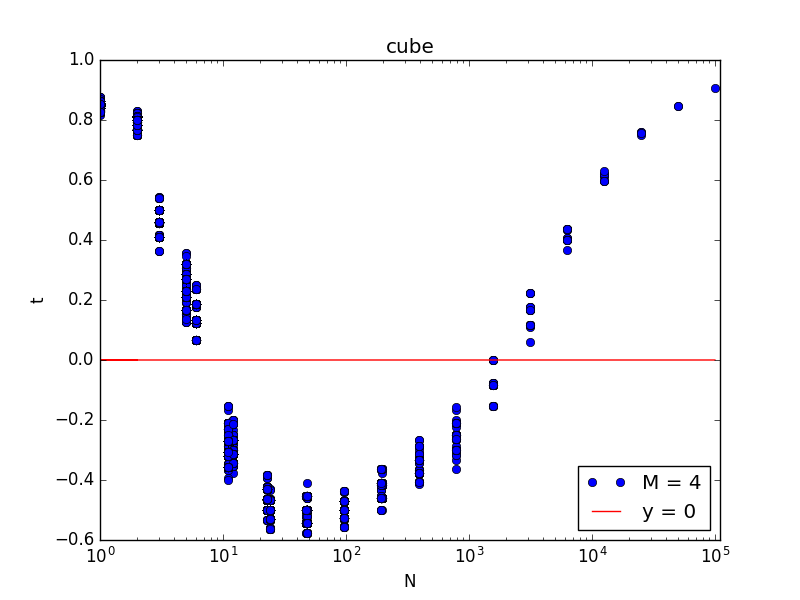
\includegraphics[width=6cm]{pic/cube_m=4}
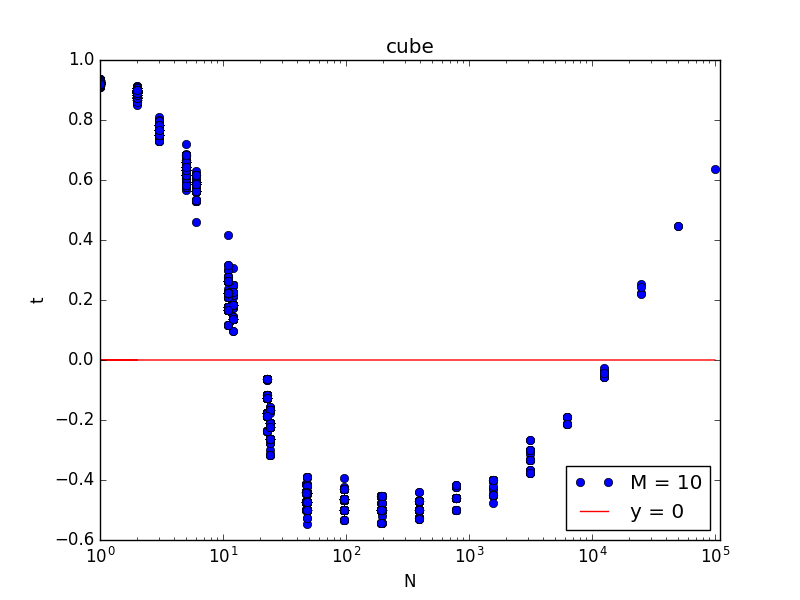
\includegraphics[width=6cm]{pic/cube_m=10}
\end{center}
\end{table}
\end{block}
\end{frame}

\begin{frame}{Практические результаты}
%\transduration{20}
\begin{block}{Случайные точки в гиперкубе}
t = $\frac{T_\text{BOS} - T_\text{Fast}}{T_\text{max}}$.
\begin{table}[h]
\begin{center}
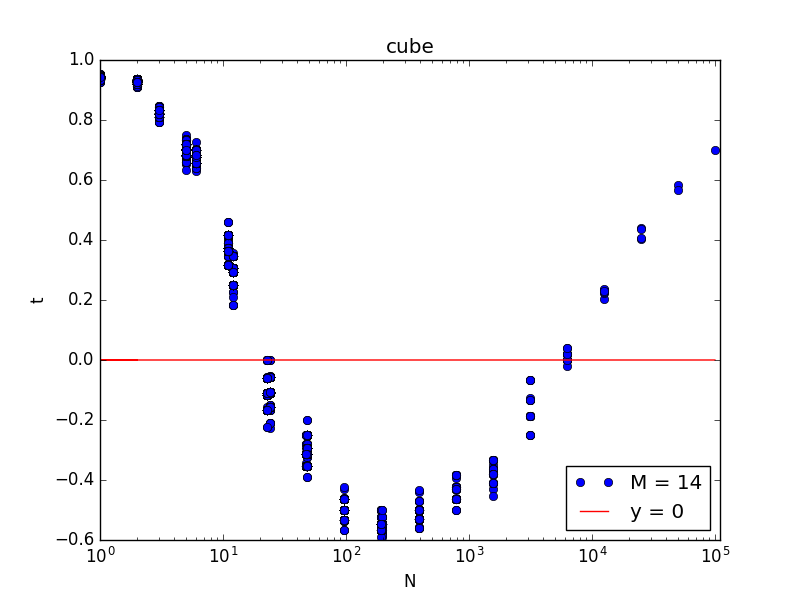
\includegraphics[width=6cm]{pic/cube_m=14}
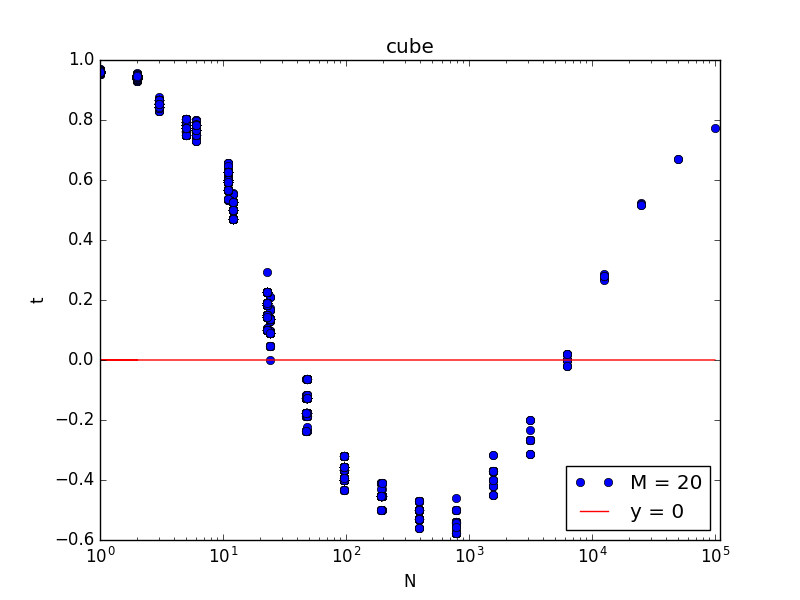
\includegraphics[width=6cm]{pic/cube_m=20}
\end{center}
\end{table}
\end{block}
\end{frame}


\begin{frame}{Практические результаты}
%\transduration{20}
\begin{block}{Случайные точки в гиперкубе}
Левая и правая границы: 
\begin{itemize}
	\item m - размерность входных данных, 
	\item n1 и n2 - размеры входных данных при которых меняется более эффективный алгоритм.
\end{itemize}
\begin{table}[h]
\begin{center}
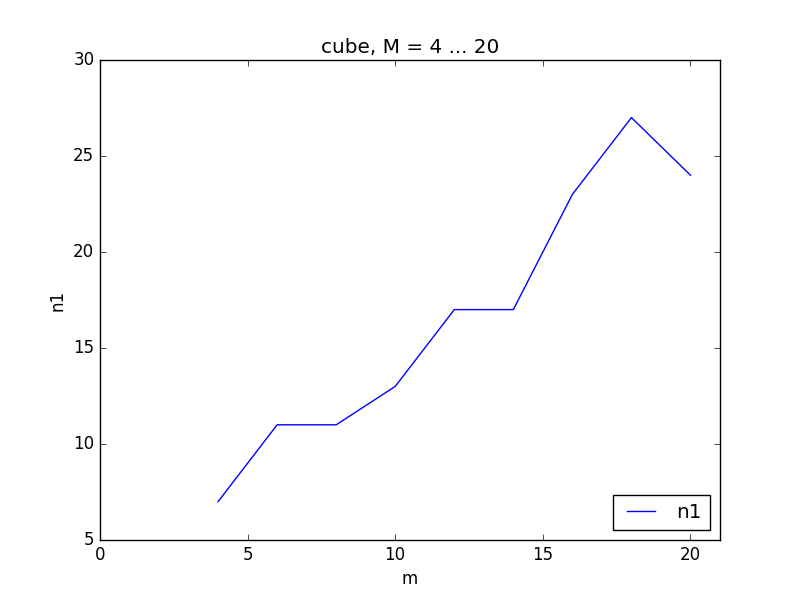
\includegraphics[width=6cm]{pic/cube_n1-}
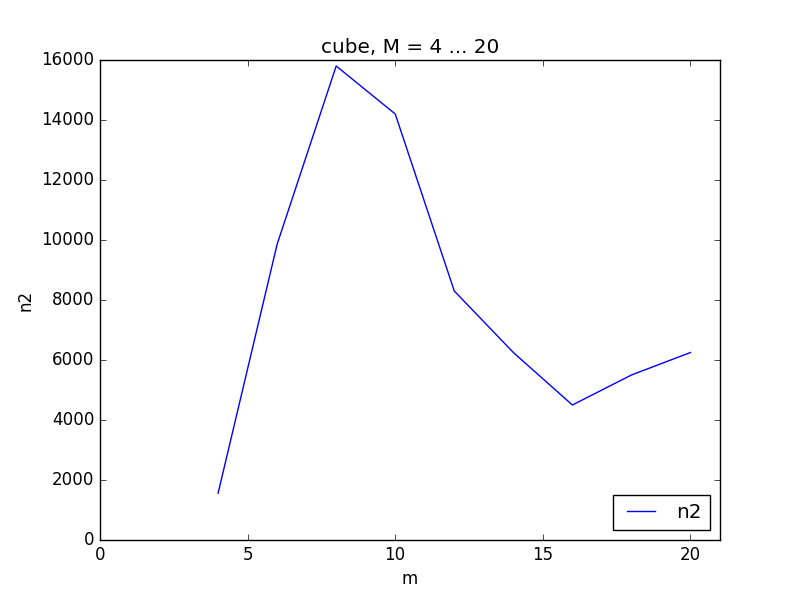
\includegraphics[width=6cm]{pic/cube_n2-}
\end{center}
\end{table}
\end{block}
\end{frame}

\begin{frame}{Практические результаты}
%\transduration{20}
\begin{block}{Точки одного ранга}
t = $\frac{T_\text{BOS} - T_\text{Fast}}{T_\text{max}}$.
\begin{table}[h]
\begin{center}
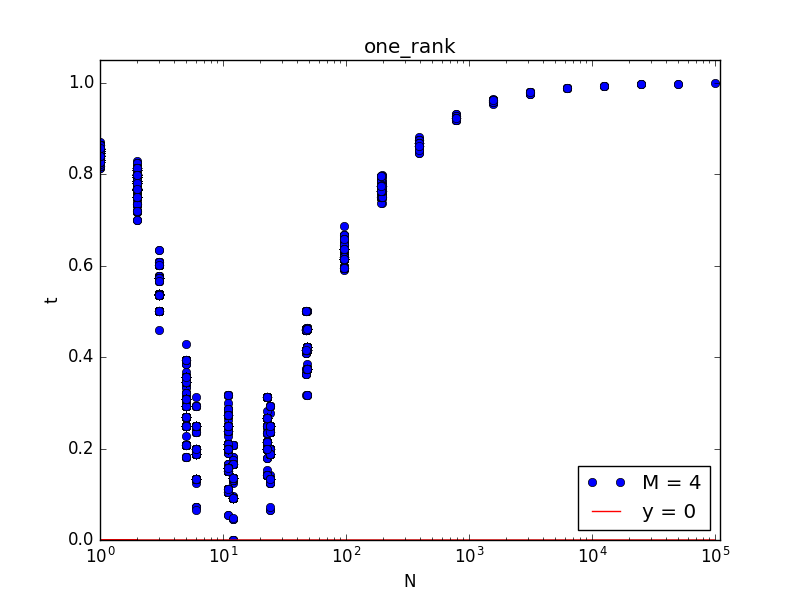
\includegraphics[width=6cm]{pic/one_rank_m=4}
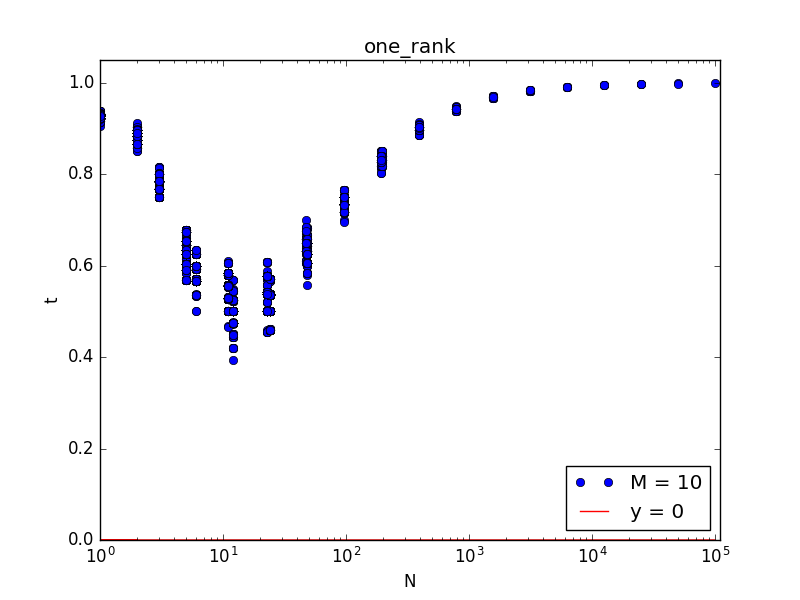
\includegraphics[width=6cm]{pic/one_rank_m=10}
\end{center}
\end{table}
\end{block}
\end{frame}

\begin{frame}{Практические результаты}
%\transduration{20}
\begin{block}{Точки одного ранга}
t = $\frac{T_\text{BOS} - T_\text{Fast}}{T_\text{max}}$.
\begin{table}[h]
\begin{center}
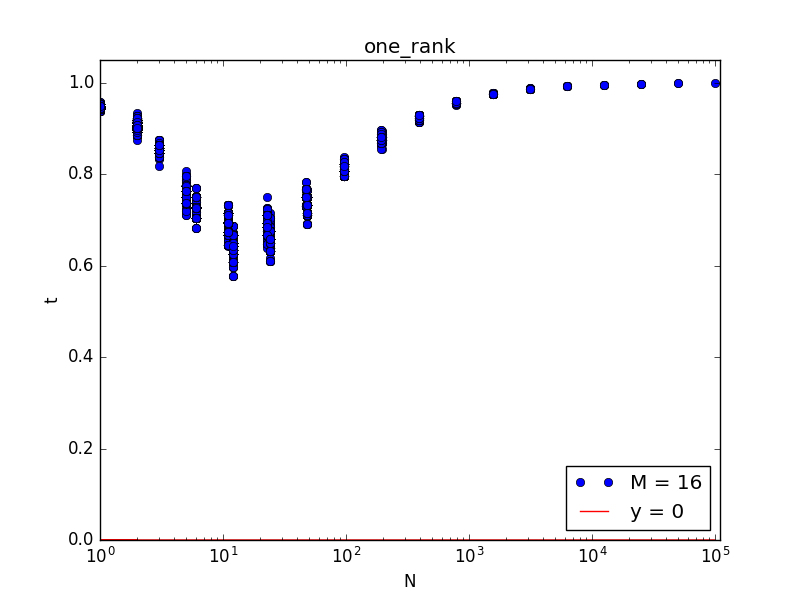
\includegraphics[width=6cm]{pic/one_rank_m=16}
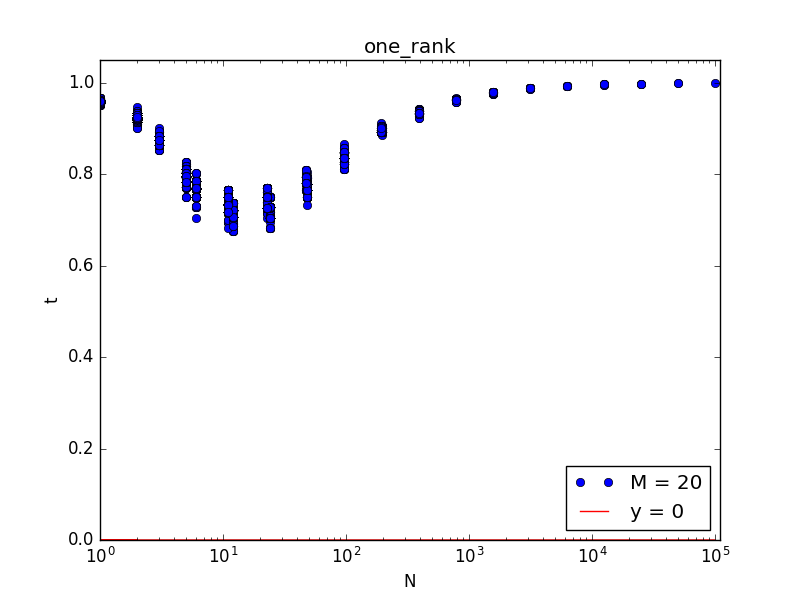
\includegraphics[width=6cm]{pic/one_rank_m=20}
\end{center}
\end{table}
\end{block}
\end{frame}

\begin{frame}{Практические результаты}
%\transduration{20}
\begin{block}{Выводы}
\begin{itemize}
	\item Стратегия выбора алгоритма, основывающаяся на размере входных данных и их размерности, будет достаточно эффективной на случайных входных данных
	\item Для более эффективной работы в крайних случаях требуется предсказывать число слоев входных данных. 
\end{itemize}
\end{block}
\end{frame}


\begin{frame}{Дальнейшие действия}
%\transduration{20}
\begin{itemize}
	\item Выявить зависимость правой границы для случайных входных данных
	\item Научиться детектировать крайние случаи и разработать стратегию выбора наиболее подходящего алгоритма для них
\end{itemize}
\end{frame}


\begin{frame}{}
\begin{center}
Спасибо за внимание!
\end{center}
\end{frame}

\appendix

\begin{frame}{Дополнительные материалы}

\end{frame}

\end{document}